\documentclass{standalone}
\usepackage[OT1]{fontenc}
\renewcommand*\familydefault{\sfdefault}
\usepackage{helvet,sfmath}
\usepackage{tikz}
\begin{document}




\tikzset{every picture/.style={line width=0.75pt}} %set default line width to 0.75pt        

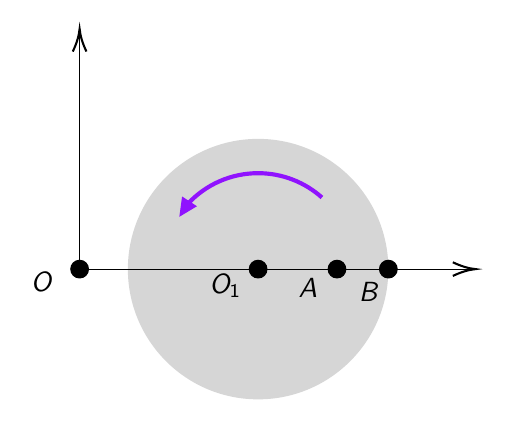
\begin{tikzpicture}[x=0.75pt,y=0.75pt,yscale=-1,xscale=1]
%uncomment if require: \path (0,15225); %set diagram left start at 0, and has height of 15225

%Shape: Circle [id:dp38627891269776693] 
\draw  [draw opacity=0][fill={rgb, 255:red, 155; green, 155; blue, 155 }  ,fill opacity=0.41 ][dash pattern={on 0.84pt off 2.51pt}] (494,5811.75) .. controls (494,5777.09) and (522.09,5749) .. (556.75,5749) .. controls (591.41,5749) and (619.5,5777.09) .. (619.5,5811.75) .. controls (619.5,5846.41) and (591.41,5874.5) .. (556.75,5874.5) .. controls (522.09,5874.5) and (494,5846.41) .. (494,5811.75) -- cycle ;
%Shape: Circle [id:dp07640531809109152] 
\draw  [fill={rgb, 255:red, 0; green, 0; blue, 0 }  ,fill opacity=1 ] (552.5,5811.75) .. controls (552.5,5809.4) and (554.4,5807.5) .. (556.75,5807.5) .. controls (559.1,5807.5) and (561,5809.4) .. (561,5811.75) .. controls (561,5814.1) and (559.1,5816) .. (556.75,5816) .. controls (554.4,5816) and (552.5,5814.1) .. (552.5,5811.75) -- cycle ;
%Straight Lines [id:da5603269254054544] 
\draw    (470.75,5811.75) -- (659.5,5811.75) ;
\draw [shift={(661.5,5811.75)}, rotate = 180] [color={rgb, 255:red, 0; green, 0; blue, 0 }  ][line width=0.75]    (10.93,-3.29) .. controls (6.95,-1.4) and (3.31,-0.3) .. (0,0) .. controls (3.31,0.3) and (6.95,1.4) .. (10.93,3.29)   ;
%Straight Lines [id:da08984703060233057] 
\draw    (470.75,5811.75) -- (470.75,5698) ;
\draw [shift={(470.75,5696)}, rotate = 90] [color={rgb, 255:red, 0; green, 0; blue, 0 }  ][line width=0.75]    (10.93,-3.29) .. controls (6.95,-1.4) and (3.31,-0.3) .. (0,0) .. controls (3.31,0.3) and (6.95,1.4) .. (10.93,3.29)   ;
%Shape: Circle [id:dp7693639958281471] 
\draw  [fill={rgb, 255:red, 0; green, 0; blue, 0 }  ,fill opacity=1 ] (590.5,5811.75) .. controls (590.5,5809.4) and (592.4,5807.5) .. (594.75,5807.5) .. controls (597.1,5807.5) and (599,5809.4) .. (599,5811.75) .. controls (599,5814.1) and (597.1,5816) .. (594.75,5816) .. controls (592.4,5816) and (590.5,5814.1) .. (590.5,5811.75) -- cycle ;
%Shape: Circle [id:dp1691604165655085] 
\draw  [fill={rgb, 255:red, 0; green, 0; blue, 0 }  ,fill opacity=1 ] (615.25,5811.75) .. controls (615.25,5809.4) and (617.15,5807.5) .. (619.5,5807.5) .. controls (621.85,5807.5) and (623.75,5809.4) .. (623.75,5811.75) .. controls (623.75,5814.1) and (621.85,5816) .. (619.5,5816) .. controls (617.15,5816) and (615.25,5814.1) .. (615.25,5811.75) -- cycle ;
%Shape: Circle [id:dp7272749619054271] 
\draw  [fill={rgb, 255:red, 0; green, 0; blue, 0 }  ,fill opacity=1 ] (466.5,5811.75) .. controls (466.5,5809.4) and (468.4,5807.5) .. (470.75,5807.5) .. controls (473.1,5807.5) and (475,5809.4) .. (475,5811.75) .. controls (475,5814.1) and (473.1,5816) .. (470.75,5816) .. controls (468.4,5816) and (466.5,5814.1) .. (466.5,5811.75) -- cycle ;
%Straight Lines [id:da7442242482064889] 
\draw [color={rgb, 255:red, 144; green, 19; blue, 254 }  ,draw opacity=1 ]   (523.01,5780.16) -- (520.44,5784.07) ;
\draw [shift={(518.79,5786.57)}, rotate = 303.35] [fill={rgb, 255:red, 144; green, 19; blue, 254 }  ,fill opacity=1 ][line width=0.08]  [draw opacity=0] (8.93,-4.29) -- (0,0) -- (8.93,4.29) -- cycle    ;
%Shape: Arc [id:dp20594200556984044] 
\draw  [draw opacity=0][line width=1.5]  (523.01,5780.16) .. controls (531.45,5771.16) and (543.44,5765.53) .. (556.75,5765.53) .. controls (568.55,5765.53) and (579.32,5769.96) .. (587.49,5777.24) -- (556.75,5811.75) -- cycle ; \draw  [color={rgb, 255:red, 144; green, 19; blue, 254 }  ,draw opacity=1 ][line width=1.5]  (523.01,5780.16) .. controls (531.45,5771.16) and (543.44,5765.53) .. (556.75,5765.53) .. controls (568.55,5765.53) and (579.32,5769.96) .. (587.49,5777.24) ;  

% Text Node
\draw (532,5813) node [anchor=north west][inner sep=0.75pt]    {$O_{1}$};
% Text Node
\draw (575,5815) node [anchor=north west][inner sep=0.75pt]    {$A$};
% Text Node
\draw (604,5817) node [anchor=north west][inner sep=0.75pt]    {$B$};
% Text Node
\draw (446,5812) node [anchor=north west][inner sep=0.75pt]    {$O$};


\end{tikzpicture}
\end{document}